% ***********************************************************
% ******************* PHYSICS HEADER ************************
% ***********************************************************
% Version 2
\documentclass[11pt]{article} 
\usepackage{amsmath} % AMS Math Package
\usepackage{amsthm} % Theorem Formatting
\usepackage{amssymb}	% Math symbols such as \mathbb
\usepackage{graphicx} % Allows for eps images
\usepackage{multicol} % Allows for multiple columns
\usepackage[dvips]{geometry}
 % Sets margins and page size
\pagestyle{empty} % Removes page numbers
\makeatletter % Need for anything that contains an @ command 
\renewcommand{\maketitle} % Redefine maketitle to conserve space
{ \begingroup \vskip 10pt \begin{center} \large {\bf \@title}
	\vskip 10pt \large \@author \hskip 20pt \@date \end{center}
  \vskip 10pt \endgroup \setcounter{footnote}{0} }
\makeatother % End of region containing @ commands
\renewcommand{\labelenumi}{(\alph{enumi})} % Use letters for enumerate
% \DeclareMathOperator{\Sample}{Sample}
\let\vaccent=\v % rename builtin command \v{} to \vaccent{}
\renewcommand{\v}[1]{\ensuremath{\mathbf{#1}}} % for vectors
\newcommand{\gv}[1]{\ensuremath{\mbox{\boldmath$ #1 $}}} 
% for vectors of Greek letters
\newcommand{\uv}[1]{\ensuremath{\mathbf{\hat{#1}}}} % for unit vector
\newcommand{\abs}[1]{\left| #1 \right|} % for absolute value
\newcommand{\avg}[1]{\left< #1 \right>} % for average
\let\underdot=\d % rename builtin command \d{} to \underdot{}
\renewcommand{\d}[2]{\frac{d #1}{d #2}} % for derivatives
\newcommand{\dd}[2]{\frac{d^2 #1}{d #2^2}} % for double derivatives
\newcommand{\pd}[2]{\frac{\partial #1}{\partial #2}} 
% for partial derivatives
\newcommand{\pdd}[2]{\frac{\partial^2 #1}{\partial #2^2}} 
% for double partial derivatives
\newcommand{\pdc}[3]{\left( \frac{\partial #1}{\partial #2}
 \right)_{#3}} % for thermodynamic partial derivatives
\newcommand{\ket}[1]{\left| #1 \right>} % for Dirac bras
\newcommand{\bra}[1]{\left< #1 \right|} % for Dirac kets
\newcommand{\braket}[2]{\left< #1 \vphantom{#2} \right|
 \left. #2 \vphantom{#1} \right>} % for Dirac brackets
\newcommand{\matrixel}[3]{\left< #1 \vphantom{#2#3} \right|
 #2 \left| #3 \vphantom{#1#2} \right>} % for Dirac matrix elements
\newcommand{\grad}[1]{\gv{\nabla} #1} % for gradient
\let\divsymb=\div % rename builtin command \div to \divsymb
\renewcommand{\div}[1]{\gv{\nabla} \cdot #1} % for divergence
\newcommand{\curl}[1]{\gv{\nabla} \times #1} % for curl
\let\baraccent=\= % rename builtin command \= to \baraccent
\renewcommand{\=}[1]{\stackrel{#1}{=}} % for putting numbers above =
\newtheorem{prop}{Proposition}
\newtheorem{thm}{Theorem}[section]
\newtheorem{lem}[thm]{Lemma}
\theoremstyle{definition}
\newtheorem{dfn}{Definition}
\theoremstyle{remark}
\newtheorem*{rmk}{Remark}

% ***********************************************************
% ********************** END HEADER *************************
% ***********************************************************

%%% Local Variables:
%%% mode: latex
%%% TeX-Master: notes
%%% End:

\usepackage[utf8]{inputenc}
\usepackage{amsmath}
\usepackage{amssymb}
\usepackage{amsfonts}
\usepackage{amssymb}
\usepackage{float}
\usepackage{indentfirst}
\usepackage{vmargin}
\usepackage{indentfirst}
\usepackage{titling}
\usepackage{color} 
\usepackage{siunitx}
\usepackage{xspace}
\usepackage{graphicx}
\usepackage{enumitem}
\usepackage[backend=biber,backref=true,style=unsrt,
style=numeric-comp,block=ragged,firstinits=true]{biblatex}
\addbibresource{ref-notes.bib}
\bibliography{ref-notes}
\graphicspath{{plot_synthesis/} {Feynman/}}

\newcommand{\mastersig}{\ensuremath{\Im{\widehat{\Sigma}^{A,B}(k,E)}}\xspace}
\newcommand{\chiqw}{\ensuremath{\Im{\chi}(q,\omega)}\xspace}

\providecommand{\norm}[1]{\lVert#1\rVert}

\newcommand{\subtitle}[1]{%
  \posttitle{%
    \par\end{center}
    \begin{center}\large#1\end{center}
    \vskip0.5em}%
}


\title{Condensed Matter II}
\subtitle{Problem set \#3}
%\author{}
\date{Spring 2014}

\begin{document}

\maketitle

\setlength{\unitlength}{1cm}
%\advance\textwidth by 3cm
%\advance\hoffset by -1.5cm 
\advance\textheight by 1cm
\advance\voffset by -1.5cm
\setmarginsrb{3cm}{0.5cm}{1.5cm}{1cm}{1cm}{1cm}{1cm}{1cm}
%\setlength{\parindent}{0cm}%

\pagestyle{plain}

\section{$T_d$ group representation}

\subsection{Background}

The group of symmetry operations of the regular tetrahedron $T_d$ is
isomorphic to the group of permutations of four objects $P(4)$.

\begin{figure}[h]
  \centering
  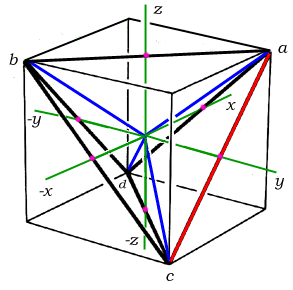
\includegraphics[width=7cm]{xyzcube.png}
  \caption{Regular tetrahedron with vertices abcd.}
\end{figure}

The elements of the group $T_d$ are (Schoenfliss notation):

\begin{itemize}
\item $E$ (identity)
\item 8 rotations  $C_3$ about the diagonals of a cube.
\item 3 rotations $C_2$ about axes $x, y , z$.
\item 6 improper rotations $S_4$ about axis $x, y , z$ (rotations
of angle $\pi/2$ followed by a reflection in a plane perpendicular to
the axis of rotation).
\item 6 reflections $\sigma_d$ in planes containing one edge and the center of
  the tetrahedron.
\end{itemize}

The elements of the group $P(4)$ are:

\begin{itemize}
\item $E=$(abcd) $A=$(acbd) $B=$(cbad) $C=$(bacd) $D=$(cabd)
  $F=$(bcad) (perm. abc;d)
\item $G=$(abdc) $H=$(adbc) $J=$(dbac) $K=$(badc) $L=$(dabc)
  $M=$(bdac) (perm. abd;c)
\item $N=$(adcb) $O=$(acdb) $P=$(cdab) $Q=$(dacb) $R=$(cadb)
  $S=$(dcab) (perm. acd;b)
\item $T=$(dbca) $U=$(dcba) $V=$(cbda) $W=$(bdca) $X=$(cdba) $Y=$(bcda) (perm. bcd;a)
\end{itemize}

\subsection{Questions}

\begin{enumerate}[label=(\roman*)]
\item Show that $P(4)$ and $T_d$ are isomorphic.
\item Determine the periods of the elements of the group.
\item Determine at least 10 subgroups.
\item Is $\{ E, G, N, T \}$ a subgroup?
\item Determine the subgroups isomorphic to $P(3)$.
\item Partition the elements of $P(4)$ so that the elements of each
  subset have the same order (the order $n$ of element $X$ is the smallest $n \in
  \mathbb{N}$ such that $X^n=E$).
\item Determine the classes (sets of equivalent elements, through the
  relation $A \sim B \Leftrightarrow \exists X \in G, B = XAX^{-1}$)
\item Find several representations.
\item Determine the irreducible representations, and the character
  table of the group.
\end{enumerate}

\end{document}